\section{Referencia de la Clase Trabajador\-View}
\label{classTrabajadorView}\index{TrabajadorView@{TrabajadorView}}
Muestra y administra la ventana con la informaci\'{o}n de un trabajador.  


{\tt \#include $<$trabajadorview.h$>$}

Diagrama de colaboraci\'{o}n para Trabajador\-View:\begin{figure}[H]
\begin{center}
\leavevmode
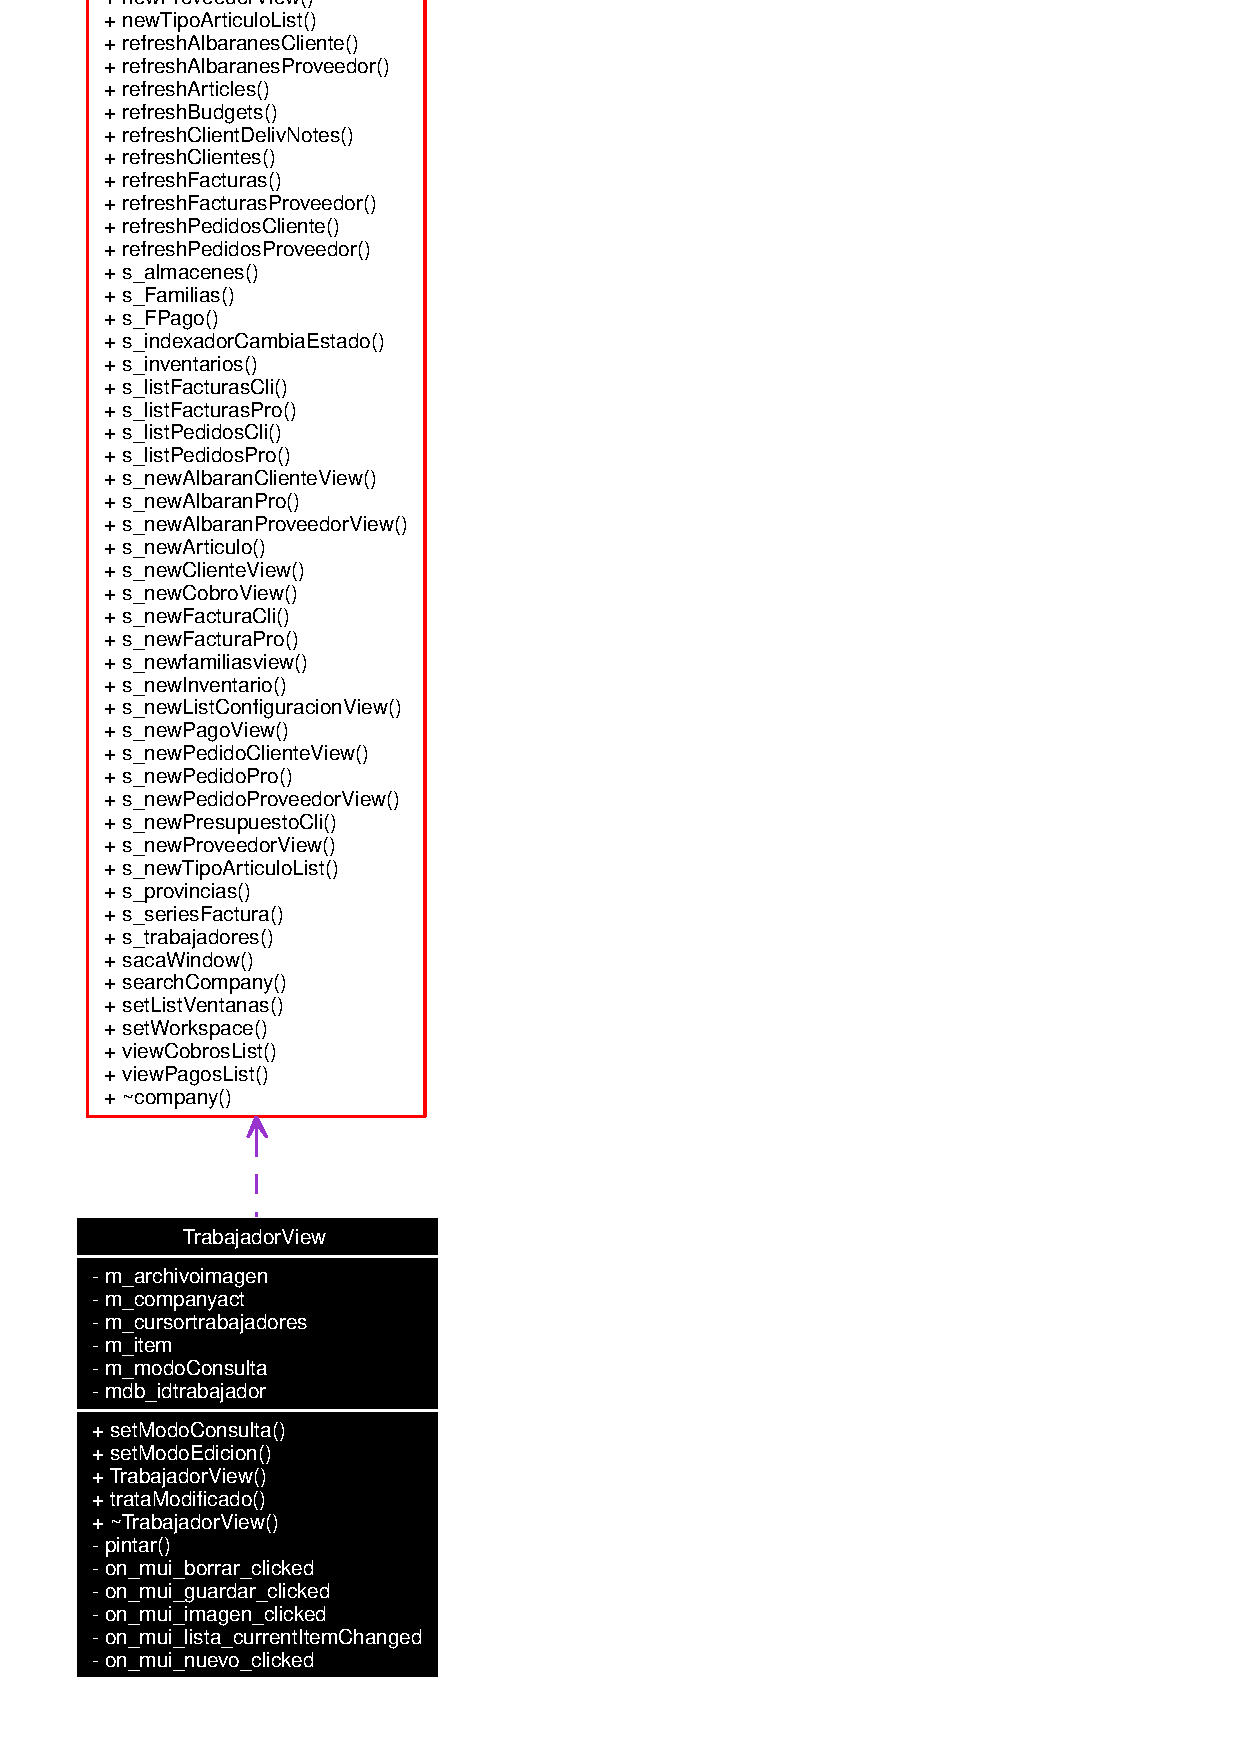
\includegraphics[width=105pt]{classTrabajadorView__coll__graph}
\end{center}
\end{figure}
\subsection*{M\'{e}todos p\'{u}blicos}
\begin{CompactItemize}
\item 
void {\bf set\-Modo\-Consulta} ()\label{classTrabajadorView_a0}

\item 
void {\bf set\-Modo\-Edicion} ()\label{classTrabajadorView_a1}

\item 
{\bf Trabajador\-View} ({\bf company} $\ast$emp, QWidget $\ast$parent=0)\label{classTrabajadorView_a2}

\begin{CompactList}\small\item\em Constructor de la clase inicializa la clase y llama a la clase de pintar para que pinte. \item\end{CompactList}\item 
bool {\bf trata\-Modificado} ()
\end{CompactItemize}


\subsection{Descripci\'{o}n detallada}
Muestra y administra la ventana con la informaci\'{o}n de un trabajador. 



\subsection{Documentaci\'{o}n de las funciones miembro}
\index{TrabajadorView@{Trabajador\-View}!trataModificado@{trataModificado}}
\index{trataModificado@{trataModificado}!TrabajadorView@{Trabajador\-View}}
\subsubsection{\setlength{\rightskip}{0pt plus 5cm}bool Trabajador\-View::trata\-Modificado ()}\label{classTrabajadorView_a3}


Si se ha modificado el contenido advertimos y guardamos. 

La documentaci\'{o}n para esta clase fu\'{e} generada a partir de los siguientes archivos:\begin{CompactItemize}
\item 
trabajadorview.h\item 
trabajadorview.cpp\end{CompactItemize}
